% ============================================================
\chapter{Matrices and Linear Maps}
\label{ch:matrices-linear-maps}
% ============================================================

\section*{Chapter Preview}
\addcontentsline{toc}{section}{Chapter Preview}

Matrices are not just rectangular tables of numbers. They represent linear
maps once bases have been chosen. This chapter connects the algebra of matrix
multiplication with the geometry of transformations.

\section{Matrices as Vector-Space Objects}

An $m\times n$ matrix over $\F$ is a rectangular array
\[
  A=(a_{ij})\in\F^{m\times n}.
\]
The set $\F^{m\times n}$ is itself a vector space: matrices of the same shape
are added entry by entry, and scalars multiply every entry.

\begin{proposition}
The vector space $\F^{m\times n}$ has dimension $mn$.
\end{proposition}

\begin{proof}
Let $E_{ij}$ be the matrix with a $1$ in position $(i,j)$ and $0$ everywhere
else. Every matrix has the unique expansion
\[
  A=\sum_{i=1}^m\sum_{j=1}^n a_{ij}E_{ij}.
\]
Thus the $mn$ matrices $E_{ij}$ form a basis.
\end{proof}

\begin{aimlbox}
A grayscale image is an $m\times n$ matrix of pixel intensities. A color image
is three such matrices. This is not only storage; it is structure. Rows,
columns, local neighborhoods, and low-rank approximations all become linear
algebraic objects.
\end{aimlbox}

\section{Matrix-Vector Multiplication}

Let $A\in\R^{m\times n}$ have columns $a_1,\ldots,a_n$. For
$x=(x_1,\ldots,x_n)^T$, define
\[
  Ax=x_1a_1+\cdots+x_na_n.
\]
Thus $Ax$ is a linear combination of the columns of $A$.

\begin{example}
If
\[
  A=\mat{1&2\\3&4\\0&1},\qquad x=\mat{5\\-1},
\]
then
\[
  Ax=5\mat{1\\3\\0}-1\mat{2\\4\\1}
    =\mat{3\\11\\-1}.
\]
\end{example}

\begin{remark}[The column-space interpretation]
The product $Ax$ can only land in the span of the columns of $A$. This simple
observation becomes the image of a linear map in Chapter~\ref{ch:image-kernel-rank-nullity}
and the existence condition for $Ax=b$ in Chapter~\ref{ch:solving-linear-systems}.
\end{remark}

\section{Linear Maps}

\begin{definition}
  A map $T:V\to W$ between vector spaces over the same field is \emph{linear}
  if
  \[
    T(u+v)=T(u)+T(v),
    \qquad
    T(\lambda v)=\lambda T(v)
  \]
  for all $u,v\in V$ and scalars $\lambda$.
\end{definition}

Equivalently, $T(\lambda u+\mu v)=\lambda T(u)+\mu T(v)$ for all choices of
$u,v,\lambda,\mu$.

\begin{proposition}
  If $A$ is an $m\times n$ matrix, then $T(x)=Ax$ is a linear map
  $\R^n\to\R^m$.
\end{proposition}

\begin{proof}
  Matrix-vector multiplication distributes over vector addition and scalar
  multiplication:
  \[
    A(u+v)=Au+Av,\qquad A(\lambda u)=\lambda Au.
  \]
\end{proof}

\section{A Linear Map Is Determined by a Basis}

If $b_1,\ldots,b_n$ is a basis of $V$, then a linear map $T:V\to W$ is
completely determined by the vectors $T(b_1),\ldots,T(b_n)$. Indeed, if
\[
  v=c_1b_1+\cdots+c_nb_n,
\]
then linearity forces
\[
  T(v)=c_1T(b_1)+\cdots+c_nT(b_n).
\]

This is why matrices work: the columns tell us where the basis vectors go.

\begin{figure}[h]
  \centering
  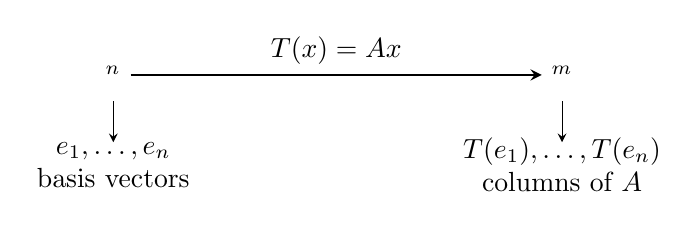
\begin{tikzpicture}[>=stealth,scale=0.95]
    \node (domain) at (0,0) {$\R^n$};
    \node (codomain) at (6,0) {$\R^m$};
    \draw[->,thick] (domain) -- node[above] {$T(x)=Ax$} (codomain);
    \node[align=center] at (0,-1.2) {$e_1,\ldots,e_n$\\basis vectors};
    \node[align=center] at (6,-1.2) {$T(e_1),\ldots,T(e_n)$\\columns of $A$};
    \draw[->] (0,-0.35) -- (0,-0.9);
    \draw[->] (6,-0.35) -- (6,-0.9);
  \end{tikzpicture}
  \caption{A matrix records where a linear map sends the basis vectors.}
\end{figure}

\section{Matrix Multiplication as Composition}

If $A:\R^n\to\R^m$ and $B:\R^m\to\R^p$, then applying $A$ and then $B$ gives
the composite map
\[
  x\mapsto B(Ax).
\]
The matrix of this composite map is $BA$.

\begin{theorem}
  Matrix multiplication represents composition of linear maps.
\end{theorem}

\begin{proof}
  The $j$-th column of the matrix of the composite is the image of the $j$-th
  standard basis vector:
  \[
    B(Ae_j).
  \]
  Since $Ae_j$ is the $j$-th column of $A$, the columns are exactly the
  columns produced by the usual definition of $BA$.
\end{proof}

\begin{proposition}[Three views of $AB$]
For compatible matrices $A$ and $B$:
\begin{enumerate}
  \item the $(i,j)$ entry of $AB$ is row $i$ of $A$ dotted with column $j$
  of $B$;
  \item the $j$-th column of $AB$ is $A$ applied to the $j$-th column of
  $B$;
  \item $AB$ is a sum of rank-one outer products.
\end{enumerate}
\end{proposition}

The column view is usually the most important one early in the course: each
column of $B$ is an input, and $A$ transforms those inputs one at a time.

\section{Differentiation as a Matrix}

Linear maps are not limited to arrows in Euclidean space. On
$\mathcal P_n$, the space of polynomials of degree at most $n$, differentiation
is linear:
\[
  D(\lambda p+\mu q)=\lambda Dp+\mu Dq.
\]
In the monomial basis $1,x,x^2,\ldots,x^n$, differentiation has a matrix:
\[
  D=
  \begin{bmatrix}
  0&1&0&\cdots&0\\
  0&0&2&\cdots&0\\
  \vdots&\vdots&\vdots&\ddots&\vdots\\
  0&0&0&\cdots&n\\
  0&0&0&\cdots&0
  \end{bmatrix}.
\]
This is a useful example because the object being transformed is a polynomial,
but the computation becomes a matrix-vector product after choosing a basis.

\section{Python: Building a Matrix from a Rule}

\begin{lstlisting}
import numpy as np

def matrix_of_T(T, n):
    cols = []
    for j in range(n):
        e = np.zeros(n)
        e[j] = 1.0
        cols.append(T(e))
    return np.column_stack(cols)

def reflect_across_y_equals_x(v):
    return np.array([v[1], v[0]])

A = matrix_of_T(reflect_across_y_equals_x, 2)
print(A)
\end{lstlisting}

\section*{Chapter Summary}
\addcontentsline{toc}{section}{Chapter Summary}

\begin{itemize}
  \item $Ax$ is a linear combination of the columns of $A$.
  \item Linear maps preserve addition and scalar multiplication.
  \item A linear map is determined by its values on a basis.
  \item Matrix multiplication represents composition.
\end{itemize}

\section*{Where This Appears Later}
\addcontentsline{toc}{section}{Where This Appears Later}

Image, kernel, rank, change of basis, eigenvalues, and SVD all build on the
idea that a matrix is a coordinate representative of a linear map.

\begin{labbox}
Lab 2 builds matrices for differentiation, integration, rotations,
reflections, projections, and composition.
\end{labbox}

\section*{Exercises}
\addcontentsline{toc}{section}{Exercises}

\subsection*{A. Theory}

\begin{exercise}
\exerciseid{4.A1}
Prove that the span of a list of vectors is a subspace.
\end{exercise}

\begin{exercise}
\exerciseid{4.A2}
Prove that if a list of vectors is linearly dependent, then at least one vector
in the list is a linear combination of the others.
\end{exercise}

\begin{exercise}
\exerciseid{4.A3}
Explain why a basis gives unique coordinates.
\end{exercise}

\subsection*{B. By Hand}

\begin{exercise}
\exerciseid{4.B1}
Do the vectors $(1,0,1)$, $(0,1,1)$, and $(1,1,2)$ form a basis of $\R^3$?
Explain without doing unnecessary arithmetic.
\end{exercise}

\begin{exercise}
\exerciseid{4.B2}
Let $b_1=(1,1)$ and $b_2=(1,-1)$. Find the coordinates of $v=(3,1)$ in the
basis $(b_1,b_2)$.
\end{exercise}

\begin{exercise}
\exerciseid{4.B3}
Find a basis for the span of
\[
  (1,2,0),\quad (2,4,0),\quad (0,1,1).
\]
\end{exercise}

\subsection*{C. Python / NumPy}

\begin{exercise}
\exerciseid{4.C1}
Put the vectors in Exercise 4.B3 into the columns of a matrix and use
\texttt{np.linalg.matrix\_rank} to check the dimension of their span.
\end{exercise}

\begin{exercise}
\exerciseid{4.C2}
Write a function \texttt{coords(B, v)} that returns the coordinate vector
$c$ solving $Bc=v$.
\end{exercise}

\subsection*{D. Challenge}

\begin{exercise}
\exerciseid{4.D1}
Give two different bases of $\mathcal P_2$ and compute the coordinates of
$p(x)=1+x+x^2$ in both bases.
\end{exercise}

